\chapter{ PROBLEMÁTICA Y ESTADO DEL ARTE DE LOS INSTRUMENTOS PARA BATERÍAS}
\section{Problemática sobre la capacidad eléctrica de las baterías}

En general, las baterías han sido muy útiles en distintos proyectos de electricidad, electrónica, robótica, entre otros. Sin embargo, la selección adecuada de una batería para cierta carga específica ha sido un problema que ha llevado a muchos usuarios, entre ellos estudiantes de pregrado, presentar consultas sobre la capacidad eléctrica de las baterías. Por ejemplo, en un foro reconocido element14, un estudiante de ingeniería eléctrica desea controlar un motor, pero no está seguro de cuánto durarían sus pilas alcalinas o si sería mejor usar una batería Li-ion~\cite{Mparmpas}. Otro ejemplo, en un foro británico reconocido, un usuario que empieza a utilizar el Raspberry Pi desea saber cuánto duraría su microcontrolador con una batería Li-ion~\cite{Elieteyssedou}. El problema de la falta de información sobre las baterías requiere mayor atención en los laboratorios donde se realizan proyectos electrónicos. Por lo tanto, urge la necesidad de realizar una estimación de la capacidad que puedan brindar las baterías. \\

Dada la gran variedad de tipos de batería en el mercado, resulta difícil obtener una estimación de la capacidad eléctrica de una batería a partir de un solo método. Incluso baterías del mismo modelo y fábrica no muestran resultados precisos usando el mismo método~\cite{Buchmann2011}. Por ello es necesario revisar los parámetros que están relacionados con la capacidad eléctrica de las baterías como, por ejemplo: impedancia interna, profundidad de descarga, temperatura, entre otros. Así mismo, se busca dar un mejor enfoque al asunto de estudio reduciendo los tipos de batería que se van a tratar en la presente tesis.

\section{Parámetros de las baterías}

Los parámetros de las baterías son aquellas variables que se utilizan para describir ciertas características que tienen en común la mayoría de baterías. Según una guía proporcionada por el equipo de vehículos eléctricos del MIT, los parámetros son divididos en dos secciones: Especificaciones técnicas de la batería y Estado de la batería. La primera sección hace referencia a las variables que se suelen encontrar en las hojas de datos de las baterías, por ejemplo: voltaje nominal, voltaje de corte, capacidad nominal, energía nominal, ciclo de vida, energía específica, entre otros. Mientras que la segunda sección hace referencia a las variables que describen la condición actual de la batería como, por ejemplo: estado de carga, profundidad de descarga, impedancia interna, entre otros~\cite{MIT-2008}. A continuación, se describe en mayor detalle los parámetros que están relacionados con la capacidad eléctrica de las baterías: \\

\textbf{\underline{Especificaciones Técnicas}}

\begin{itemize}
\item \underline{Profundidad de Descarga:} La profundidad de descarga, también conocido como Depth of Discharge (DoD), se refiere al porcentaje de la capacidad máxima de la batería que ha sido descargado~\cite{MIT-2008}. Así mismo, el DoD es un indicador que está estrechamente relacionado con el ciclo de descarga y el voltaje de fin de descarga. Este último indica el voltaje límite de la batería donde ya no se pueda descargar más, ya que se utiliza como medio de protección para evitar sobre descargas que dañen la batería. Así mismo, cabe resaltar que el voltaje de fin de descarga es afectado si es que la batería es descargada a corrientes altas o la temperatura es considerablemente alta o baja.

\begin{table}[htbp]
\caption{Voltajes de fin de Descarga para distintos tipos de batería y a diferentes cargas~\cite{Buchmann2011}.}
\begin{center}
\begin{tabular}{|c|c|c|c|c|}
\hline
\textbf{End-of-discharge} &  \textbf{Li-manganese} & \textbf{Li-phosphate} & \textbf{Lead Acid} & \textbf{NiCd/NiMH} \\
\hline
Normal load & 3.00 V/cell & 2.70 V/cell & 1.75 V/cell & 1.00 V/cell \\
\hline
Heavy load & 2.70 V/cell & 2.45 V/cell & 1.40 V/cell & 0.90 V/cell \\
\hline
\end{tabular}
\end{center}
\label{tab:batcarga}
\end{table}

En la tabla~\ref{tab:batcarga} se puede apreciar los diferentes niveles de voltaje que se encuentra las baterías una vez descargadas, estos datos sirven como referencia para los instrumentos de medición.

\item \underline{Ciclo de Descarga:} El ciclo de descarga se debería entender que es el ciclo de carga y descarga total de la batería; sin embargo, los fabricantes de baterías, por lo general, tienden a establecer que solo se utilice un 80\% de profundidad de descarga y el otro 20\% queda como reserva. La razón por la que los fabricantes establecen esta medida es debido a que una descarga incompleta incrementa el tiempo de vida de la batería. No existen estándares fijos que constituyan un ciclo de descarga, no obstante, las baterías inteligentes consideran que un ciclo de descarga no debería ser menor a 70\%. Además, en términos de ciclo de carga y descarga, la capacidad eléctrica de las baterías se ve afectada, ya que reduce su desempeño considerando el tipo de descarga que se haya realizado~\cite{Buchmann2011}.

\begin{figure}[htbp]
\begin{center}
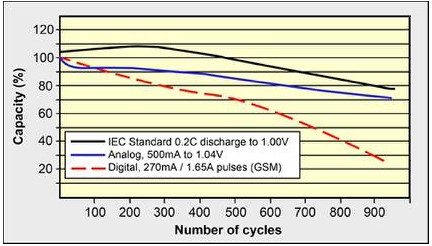
\includegraphics[width=12cm]{CAP1_curvabaterianimh.jpg}
\caption{Ciclo de vida de una batería Níquel Metal Hidruro(Ni-MH) bajo diferentes tipo de descarga~\cite{Buchmann2011}.}
\label{fig:baterianimh}
\end{center}
\end{figure}

En la figura~\ref{fig:baterianimh} se puede observar que las descargas por pulsos afectan demasiado a la capacidad eléctrica de las baterías, generalmente este tipo de descarga se encuentra en los celulares. Por otro lado, se percibe que las descargas a ratio C estandarizado por IEC y las descargas analógicas no afectan en gran magnitud a los ciclos de carga y descarga de la batería. Por último, resaltar que las pruebas de la ilustración 1 son de una batería Níquel Metal Hidruro(Ni-MH), sin embargo, el autor señala que el comportamiento es similar para las baterías Li-ion~\cite{Buchmann2011}.

\item \underline{Capacidad nominal:} La capacidad nominal de una batería es la cantidad de energía que puede proveer a los sistemas y es medido en mili Ampere-hora (mAh). Esta medida indica la cantidad de tiempo que puede durar una batería siendo descargada a una cantidad de corriente. Por ejemplo, una batería que indica una capacidad nominal de 2000mAh es capaz de cargarse o descargarse en una hora a una corriente de 1 Amperio. Sin embargo, cabe resaltar que en la práctica esto no sucede ya que hay otros factores como temperatura, impedancia interna, nivel de corriente, tipo de batería y entre otros que afectan la capacidad nominal~\cite{Buchmann2011},~\cite{MIT-2008}.

\end{itemize}

\textbf{\underline{Estado de la batería}}

\begin{itemize}

\item \underline{Estado de la carga:}El estado de carga, también llamado State of Charge (SoC), es un parámetro de la batería que se expresa en porcentaje e indica la capacidad eléctrica que puede proveer una batería sobre su capacidad nominal. El SoC, por lo general, es calculado usando una integración de cargas aplicada como corriente para determinar el cambio de la capacidad eléctrica de la batería en el tiempo~\cite{MIT-2008}. Así mismo, el parámetro SoC es exactamente lo contrario al DoD, por lo que es válido afirmar sobre un SoC mínimo del 20\% para evitar daños a la batería~\cite{FerrerAlayeto2011}. \[SoC_{min} = 100\% - DoD_{max}\] Los métodos más utilizados para determinar el SoC son tres: Medición de la densidad específica, Medición basada en la tensión, Coulomb Counting y la combinación de técnicas recién mencionadas. Sin embargo, como el objetivo de la tesis no es estimar la capacidad eléctrica de la batería durante su tiempo de vida estimada, no se entrará en detalle de estas técnicas.

\item \underline{Impedancia Interna:} La impedancia interna es la resistencia que oponen todos los componentes internos de la batería como electrodos electrolito y terminales~\cite{FerrerAlayeto2011}. Además, la resistencia interna varía en función del estado de carga, estado de salud y el tipo de batería que se está analizando. A medida que la resistencia interna sube, la eficiencia de la batería disminuye y la estabilidad térmica se reduce de manera proporcional a la carga de energía que se convierte en calor~\cite{MIT-2008}. Según Isidor Buchmann, usualmente se utiliza como referencia la impedancia interna para cambiar las baterías, ya que si ésta es muy alta significa que la batería esta por caducar. Sin embargo, este método es especialmente útil para baterías estacionarias como las baterías plomo ácido~\cite{Buchmann2011}.

\end{itemize}

\textbf{\underline{Temperatura}}

Las descargas varían el desempeño de las baterías según su tipo, además de eso las descargas también afectan a las baterías si son realizadas a diferentes temperaturas. En el libro Batteries in a Portable World, el autor afirma que las baterías, que operan a altas temperaturas, aumentan su desempeño mediante la reducción de su impedancia interna y acelerando los metabolismos químicos; sin embargo, esto reduce su tiempo de vida. En adición, el autor sostiene que cuando las baterías operan a bajas temperaturas, se incrementa su impedancia interna y disminuye su capacidad eléctrica. Si una batería podía entregar el 100\% de su capacidad a una temperatura de 27\degree C, se estimaría que entregaría solo el 50\% a -18\degree C~\cite{Buchmann2011}. 

\section{Tipos de batería}

Luego de revisar los diferentes parámetros de las baterías, se observó que éstos difieren mucho entre los distintos tipos de batería. Por lo tanto, para el objetivo de la tesis se reducirá el campo de estudio del instrumento a las baterías que se vendan más en el mercado o los más utilizados en los proyectos manejados en los laboratorios.

\begin{figure}[htbp]
\begin{center}
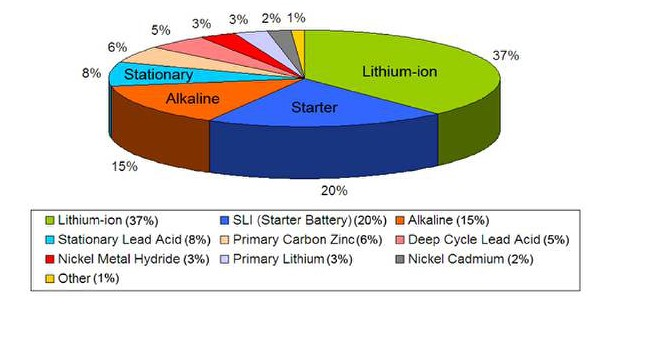
\includegraphics[width=12cm]{CAP1_frostsullivan.jpg}
\caption{Frost Sullivan (2009) - Contribuciones de ingresos clasificados por tipo de batería~\cite{Buchmann2011}.}
\label{fig:frostsullivan}
\end{center}
\end{figure}

Según un estudio realizado el 2009 por Frost Sullivan, habían pronosticado que las baterías primarias (no recargables) iban a decaer en un 7.4\% en el mercado con proyección al 2015, ya que las baterías secundarías (recargables) las estaban desplazando. Así mismo, en la figura~\ref{fig:frostsullivan}, se observa que hay 3 tipos de baterías predominantes en el mercado: las baterías li-ion, las baterías de arranque y las baterías alcalinas. Las baterías li-ion y alcalinas son muy comunes en los proyectos utilizados por los estudiantes, profesores o investigadores debido a su peso liviano y duración apropiada. Sin embargo, las baterías de arranque son baterías utilizadas en los automóviles o sistemas pesados en la industria. Por lo tanto, a partir de este punto, el campo de estudio de la tesis abarcará a las baterías li-ion y baterías alcalinas, también llamadas pilas alcalinas en el mercado local.

\section{Objetivos}

\subsection{Objetivo General}

Diseñar y desarrollar un instrumento que permita estimar la capacidad eléctrica que proveen los bancos de baterías basados en baterías tipo li-ion, como las que se emplean en para teléfonos móviles, y pilas alcalinas.

\subsection{Objetivos Específicos}

Para el desarrollo de este trabajo de tesis se tuvo que cumplir con los siguientes objetivos:

\begin{enumerate}[label=(\alph*)]
\item Estudio previo sobre conceptos de medición y métodos para la estimación de la capacidad eléctrica de las baterías.
\item Diseño e implementación de un prototipo del instrumento de medición.
\item Desarrollo del software para el control de descarga de corriente constante.
\item Programación de la interfaz con el usuario.
\item Realizar pruebas del prototipo para mostrar las curvas de descarga de la batería.
\end{enumerate}

